

\documentclass{acm_proc_article-sp}


\usepackage{graphicx}
\usepackage{listing}
\usepackage{listings} \lstset{basicstyle=\tiny,numbers=none, breaklines=true, numberstyle=\tiny, numbersep=5pt,firstnumber=last,language=XML,escapeinside={(*@}{@*)} }  

% *** CITATION PACKAGES ***
%
\usepackage{cite}
\usepackage{url}
%\usepackage[scaled=point85]{luximono}
\hyphenation{op-tical net-works semi-conduc-tor name-space}

\begin{document}

\title{VIENNA Add-In \\ Visualizing Inter-ENterprise Network Architectures}


%Do not change this number
\numberofauthors{2}


\author{
% You can go ahead and credit any number of authors here,
% e.g. one 'row of three' or two rows (consisting of one row of three
% and a second row of one, two or three).
%
% The command \alignauthor (no curly braces needed) should
% precede each author name, affiliation/snail-mail address and
% e-mail address. Additionally, tag each line of
% affiliation/address with \affaddr, and tag the
% e-mail address with \email.
%
% 1st. author
\alignauthor
Christian Huemer, Philipp Liegl, Thomas Motal, Rainer Schuster, Marco Zapletal \\
       \affaddr{Vienna University of Technology}\\
       \affaddr{Favoritenstrasse 9-11/188}\\
       \affaddr{1040 Vienna, Austria}\\
       \email{\{firstname.lastname\}@tuwien.ac.at}       
\alignauthor
Christian Eis, Martina Hiesinger, Fabian Kromer, Robert Kromer, Andreas Kuntner, Christian Pichler, Michael Strommer\\
       \affaddr{Research Studios Austria}\\
       \affaddr{Thurngasse 8/3/20}\\
       \affaddr{1090 Vienna, Austria}\\
       \email{\{firstname.lastname\}@researchstudio.at}       
% 2nd. author
%\alignauthor
%Christian Pichler\\
%       \affaddr{Research Studios Austria}\\
%       \affaddr{Thurngasse 8/3/20}\\
%       \affaddr{1090 Vienna, Austria}\\
%       \email{cpichler@researchstudio.at}
}

\date{28 April 2009}

\maketitle
\begin{abstract}

%What is the problem
The definition of concise and interoperable business documents has become one of the key issues in electronic business transactions. 
In this paper, we present our tool VIENNA Add-In supporting a business document modeler in creating Core Component compliant business document models using the Unified Modeling Language (UML). The Core Components standard defines reusable building blocks for constructing business documents and is maintained by UN/CEFACT (United Nations Center for Trade Facilitation and Electronic Business). Our tool provides a set of powerful features for Core Components such as model validation, semi-automatic generation of model artifacts, and generation of fully compliant XML Schema definitions from a conceptual model representation. Thereby, the VIENNA Add-In helps to shorten development cycles and reduces errors in designing business documents. The overall goal of our tool-based approach for inter-organizational processes is the generation of deployment artifacts for IT systems from conceptual models.


\end{abstract}
% A category with the (minimum) three required fields
\category{H.4}{Information Systems Applications}{Miscellaneous}
\terms{Business document modeling, conceptual modeling, XML schema generation}

\section{Introduction}
Before two business partners engage in an automated Business-to-Business (B2B) interaction two agreements have to be made. First, the process choreography has to be specified, i.e., the exact exchange order of the different business documents. Second, the business information being exchanged in the electronic transaction must be specified, i.e., the business document definition. In a joint effort between the Vienna University of Technology\footnote{http://www.tuwien.ac.at/} and the Research Studios Austria, Studio Inter-Organisational Systems\footnote{http://ios.researchstudio.at/}, we have developed the VIENNA Add-In \cite{man:VIENNAAddIn}. The Add-In is built on top of the UML modeling tool Enterprise Architect (EA) from Sparx Systems. %\footnote{http://www.sparxsystems.com.au}.
\begin{figure}[htbp]
 \centering
   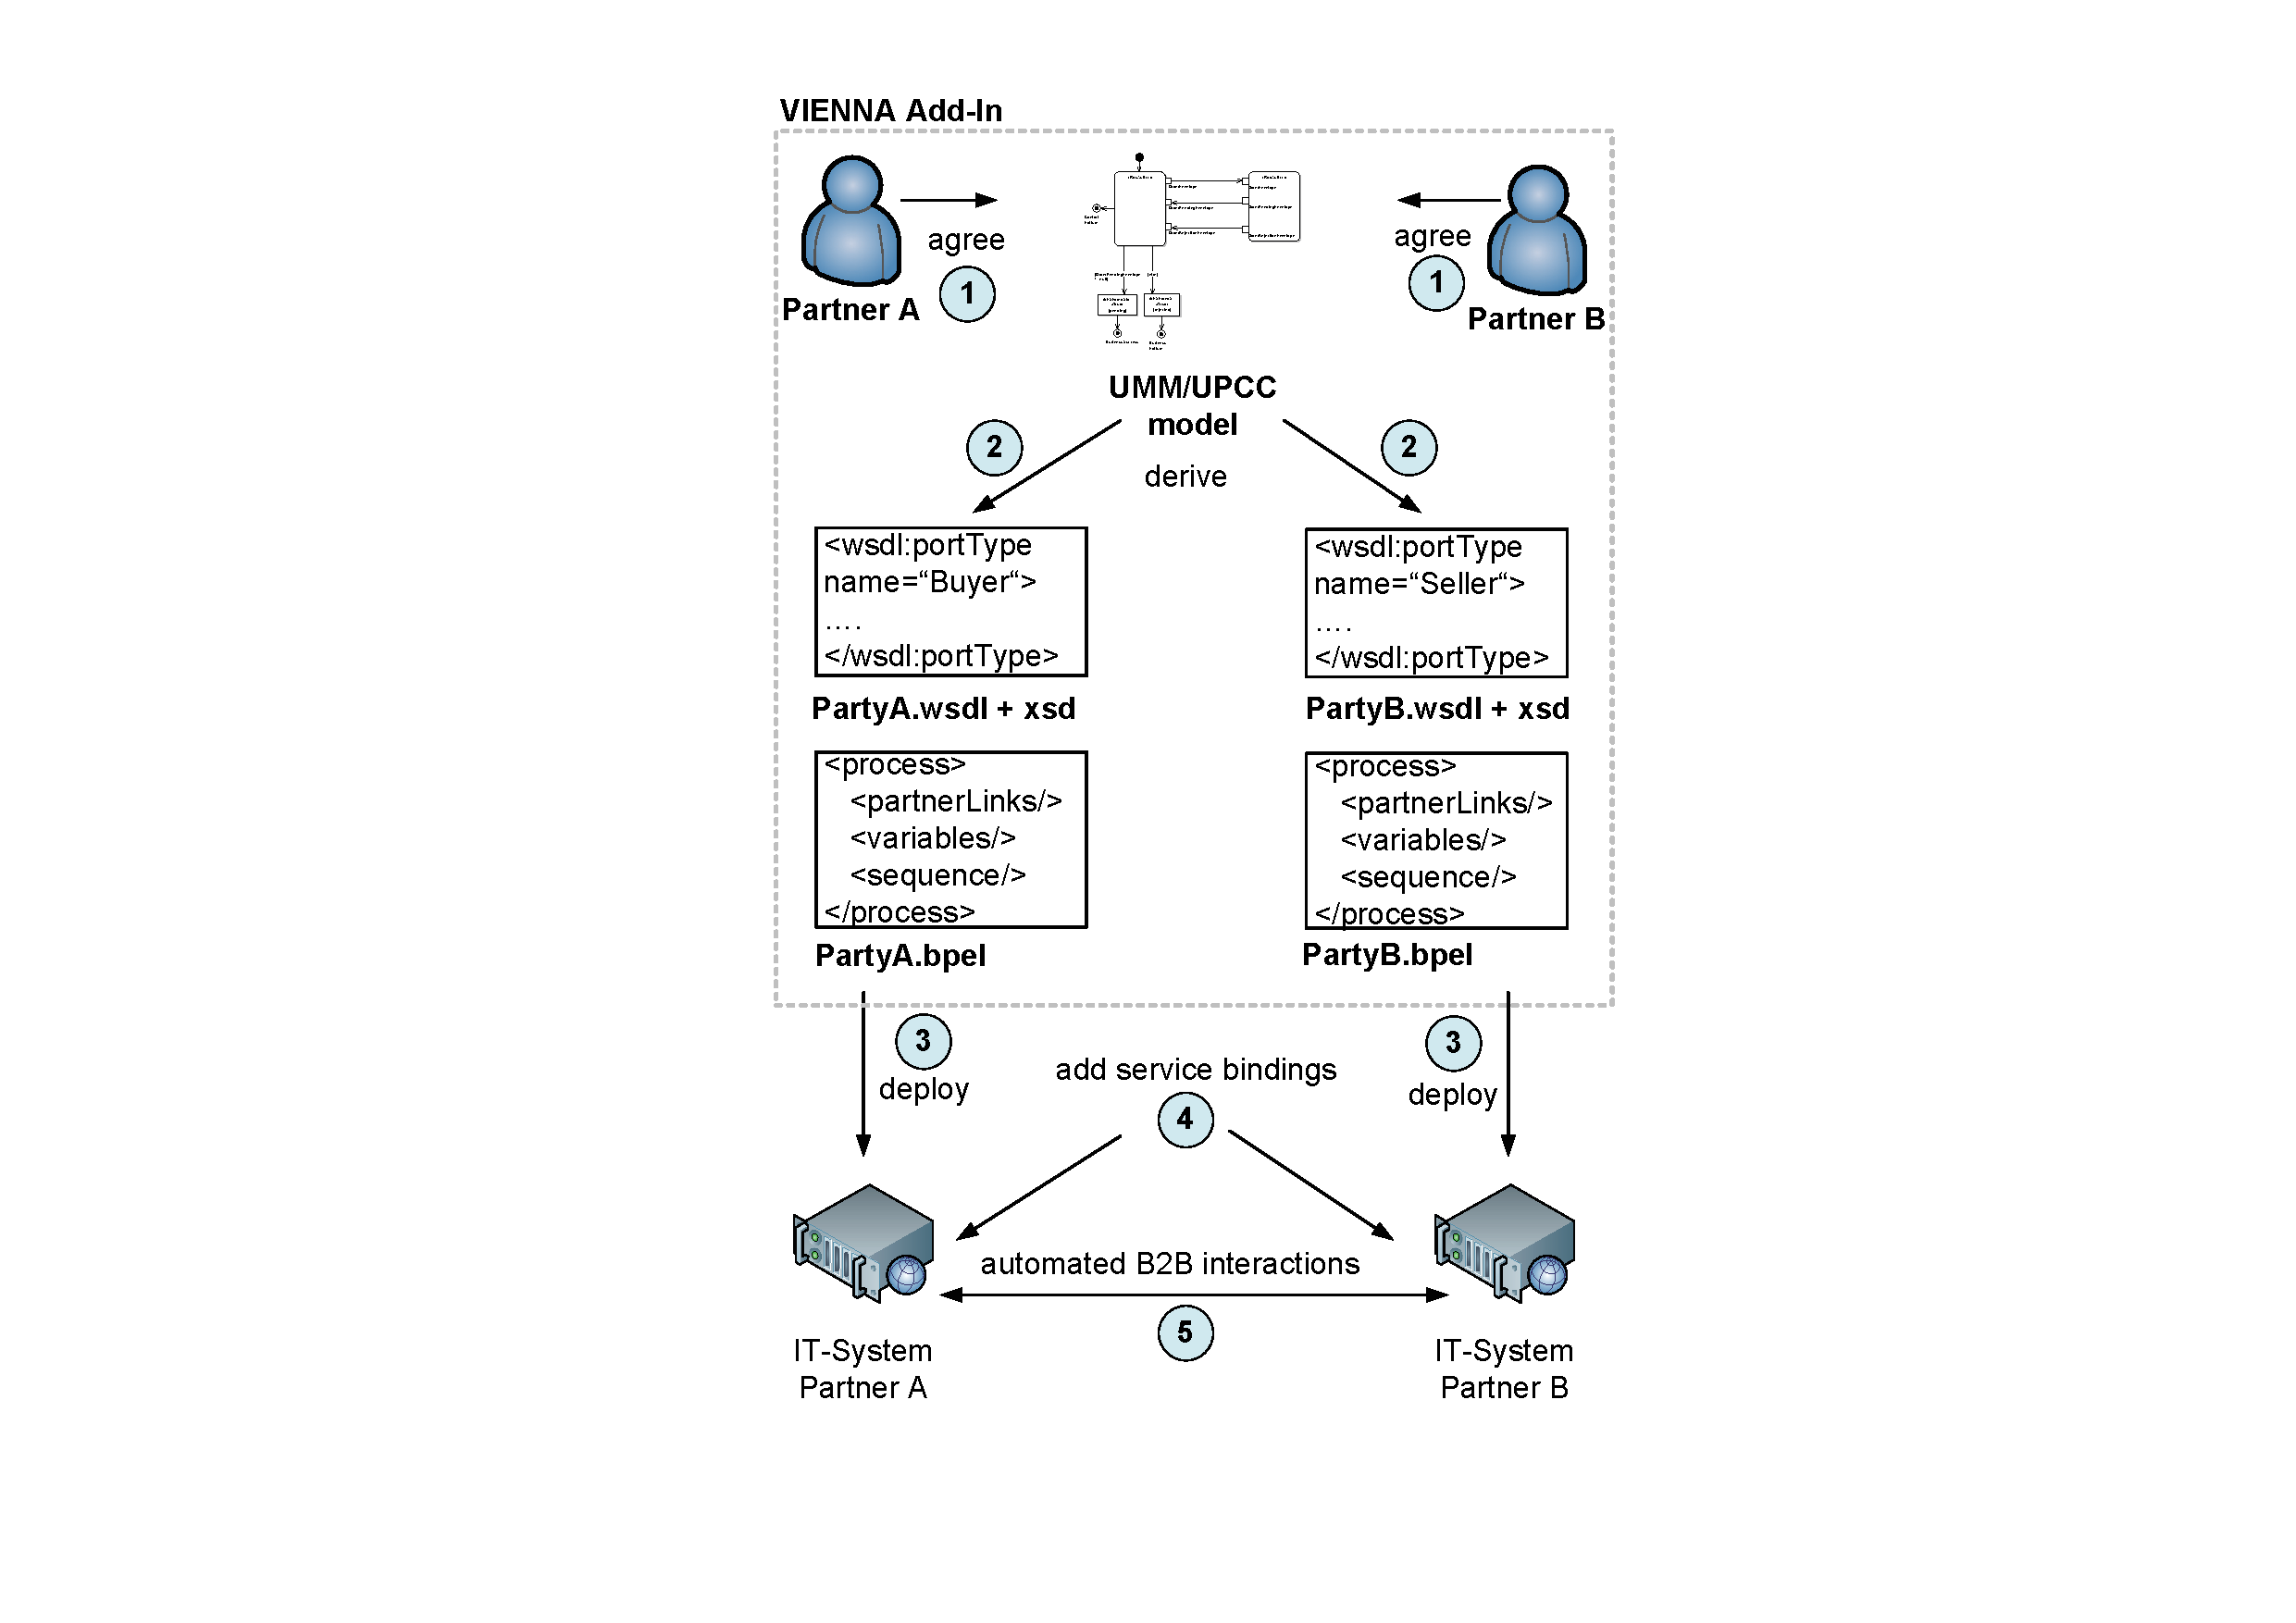
\includegraphics[width=0.32\textwidth]{figures/addinoverview.pdf}
 \caption{VIENNA Add-In overview}
 \label{fig:viennaaddinoverview}
\end{figure}
The VIENNA Add-In currently supports both, business choreography definitions and business document definitions. For the former the supported approach is UN/CEFACT's Modeling Methodology (UMM) \cite{man:umm2} and for the latter the UML Profile for UN/CEFACT's Core Components (UPCC) \cite{man:upcc}. Both UML profiles tailor the UML to the specific needs of business process modeling and business document modeling, respectively. \\Figure \ref{fig:viennaaddinoverview} gives a brief overview of the main approach pursued by the VIENNA Add-In. Two business partners willing to engage in an electronic collaboration first agree on a common UMM model specifying the business choreography and a common UPCC model specifying the exchanged business information (see (1) in Figure \ref{fig:viennaaddinoverview}). In a consecutive step the commonly agreed upon process and information model is used to derive deployment artifacts for the IT systems (2). Interface definitions and the exchanged information are reflected using WSDL and XML Schema artifacts. The local choreography definitions are reflected using Business Process Execution Language (BPEL) artifacts. Finally the generated artifacts are deployed to \textit{business service interfaces} (3). After adding service bindings (4) automatic B2B interactions are feasible (5). Thus, the business modeler is provided with a model driven approach for the definition of deployment artifacts for service oriented systems. Since the deployment artifacts for both business partners are derived from a common conceptual model, the business document definitions and process choreography definitions on both sides match. The following three sections outline three of the core features of the VIENNA Add-In.


\section{UML Profile Definition}
 
Within Enterprise Architect users may extend the standard UML modeling features through utilizing so-called \textit{model driven generation} (MDG) technologies which are an EA specific extension mechanism. An MDG technology is a set of collected resources, such as UML profiles, UML patterns, customizations for toolbox and diagram definitions, and quick link definitions, bundled into an XML file. We created MDG technologies for UMM and UPCC in order to support business process modeling and business document modeling in Enterprise Architect. Both MDG technology files are provided online\footnote{UMM: http://www.umm-dev.org/ea/umm2.xml\\UPCC:\; http://www.umm-dev.org/ea/upcc3.xml}. After successful configuration of EA these MDG technologies are dynamically loaded during every EA startup. Dynamic loading provides a suitable solution in order to keep the technology automatically up-to-date to the most recent version. \\
In order to provide a modeling environment shaped to the specific needs of UMM and UPCC we customized toolbox and diagram definitions. Toolbox definitions restrict the generic UML toolboxes to the modeling elements defined in UMM and UPCC. Both, UMM and UPCC comprise different toolbox definitions, split according to the respective artifacts. Custom diagram definitions for the different artifacts allow to automatically display the appropriate toolbox, depending on the model artifact currently being worked on.
Furthermore we use the \textit{quick link} feature for a context driven creation of new elements and relationships. Depending on the modeling element selected on the modeling canvas, only the allowed relationships are offered to the user. The proposed relationship may be used in a twofold manner. Either the relationship is drawn to an existing item or, depending on the selected source element and the relationship type, a new target element may be created.

\section{Semi-automatic artifact generation}

In our tool demonstration we will in particular focus on the business document specific features. The typical approach to model business documents involves three steps. First a generic model, using context independent core components is created. Core components are reusable building blocks for assembling business document reference models. Standardized core component definitions are retrieved from a shared library, maintained by UN/CEFACT. In a second step the business document modeler starts to derive context specific business information entities from core components. Business information entities are always derived from core components by restriction, thus every business information entity has a common semantic basis, namely the underlying core component. Finally, the third step is the derivation of XML schema artifacts from the conceptual core component models which will be covered in the next section. \\Especially the derivation of artifacts on the business information entity level involves simple, but repetitive modeling tasks. Therefore, we implemented a set of wizards supporting the user in performing these tasks. At the moment, these features include a wizard for creating a default library structure as specified in the UPCC, a wizard for importing the standard core component libraries published by UN/CEFACT, a wizard for deriving business information entities from core components, as well as a wizard guiding the user through the process of generating XML Schema artifacts. The generation of XML Schema artifacts is described in more detail in the following. 

\section{XML Schema generation}
In order to use the core component models composed with UPCC in a real world business process we provide the VIENNA Add-In with an XML Schema generator. The derivation of XML Schema files is driven by the general Naming and Design Rules (NDR) provided by UN/CEFACT \cite{CEFACT:NDR}. These Naming and Design Rules constitute a mapping between the conceptual model and the XML Schema language. Thus, it is ensured that models conforming to these rules are interchangeable across platforms and applications. For every business document a set of XML Schema files is created, reflecting the library structure of a standard UPCC model. For example, for an assembled business document in a document library, the libraries on the business information entity level are stored in separate files as well. Following the specification in \cite{CEFACT:NDR} element annotations containing meaningful documentation are generated from values of the conceptual model as well. \\Until now the VIENNA Add-In only supports the generation of XML schemas conforming to the UN/CEFACT NDR. However, it is desirable to have schema generators for other XML schema formats too. Future work concentrates on the implementation of additional schema generators and on the implementation of mapping features for matching different document models.


\bibliographystyle{abbrv}
\bibliography{references}  
\end{document}
